\clearpage
\begin{flushright}
	\textit{Лекция №4}
	\textit{2016.03.14}
\end{flushright}

Буферизация - ???

Кеширование – предназначено для хранения актуальной информации об объектах, с которыми работает пользователь, чтобы избежать обращения к диску.

open – находится в $fsopen.c$, первое что делает, это вызывает \verb|sysopen()|. 

\lstinputlisting[language=c, caption=Функции sysopen и filp\_open]{listing/1.c} 

\verb|open_namei| используется для генерации структуры \verb|nameidata nd|. Эта структура выполняет ряд действий и в конечном итоге линкует inode файла. Потом вызывается \verb|dentry_open| (dentry – вход в директорию). В результате мы должны различать не только inode и file, еще и должны отличать dentry. Ф-я  \verb|dentry_open| спускается в соответствии с указанным путем по дереву каталогу. Спуск продолжается пока не будет получен требуемый файл или пока не поймем, что файл получен никогда не будет. Если каждый компонент пути был кеширован (как dentry), то скорость будет быстрая, так как все действия выполняются в памяти. При этом, если в результате inode прочитан, то увеличивается его счетчик ссылок. Если счетчик = 0 и inode не грязный, то он удаляется из списка \verb|inodeunused| и вставляется в список. Если файл не был объектом доступа ранее, то его inode кеширован не был. В этом случае inode будет прочитан с уровня файловой системы и в результате будет кеширован. 

Рассмотрим как осущетсвляется процесс кеширования. Сначала вызывается функция \verb|get_new_inode()|  которая выделяет память под новый inode и получает на неё указатель. Память выделяется в хеш-таблице. В \verb|inode_cachep| \verb|get_new_inode()| может устанавливать блокировку. Поэтому, чтобы не войти в дедлок, ф-я должна сбросить спин блокировку inode block. Эта блокировка устанавливает, чтобы не было одновременного доступа разных процессов к одному и тому же inode. Поэтому функция должна сбросить спин блокировку, затем поиск в хеш таблице повторяется. Если на этот раз inode найден, то вновь созданный – будет удален. Если он не был найден, то вновь созданный inode будет использоваться и он инициализируется соответствующими параметрами. 
\verb|dentry_open()| размещает новую структуру \verb|file| и связывает с \verb|dentry| и \verb|fvsmount|, после чего вызывает метод \verb|f_po->open()| который был определен в \verb|inode->i_fop| при чтении inode функцией \verb|open_namei()|

\lstinputlisting[language=c, caption=Функции dentry\_open]{listing/2.c} 

\verb|dentry_open()| находит адрес функции на уровне файловой системы, необходимо найти функцию, которая откроет файл. И это будет функция контркретной файловой системы.Сначала надо найти какой файловой системе принадлежит открываемый файл, найти его inode и уже для файлов данной файловой системы определяется соответствующая функция \verb|open()|. Поэтому, чтобы найти адрес фукнции на уровен файловой системы, которая может открыть, ей надо передать inode и созданную структуру file. 
Адрес функции находится или в самом inode или в одном из родительских inode'ах.

\begin{figure}[H]
  \centering
  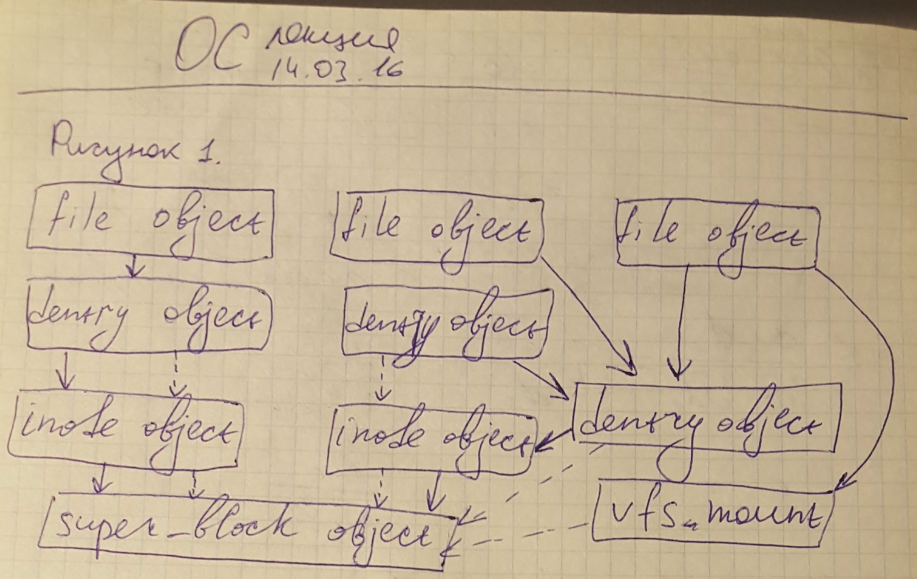
\includegraphics[width=\textwidth]{pic/1.png}
  \caption{pic}
\end{figure}

\lstinputlisting[language=c, caption=Структуры dentry и vfsmount]{listing/3.c} 

Объект dentry не соответствует какой либо структуре данных на жестком диске. Создает на основании строкового имени пути.

\begin{figure}[H]
  \centering
  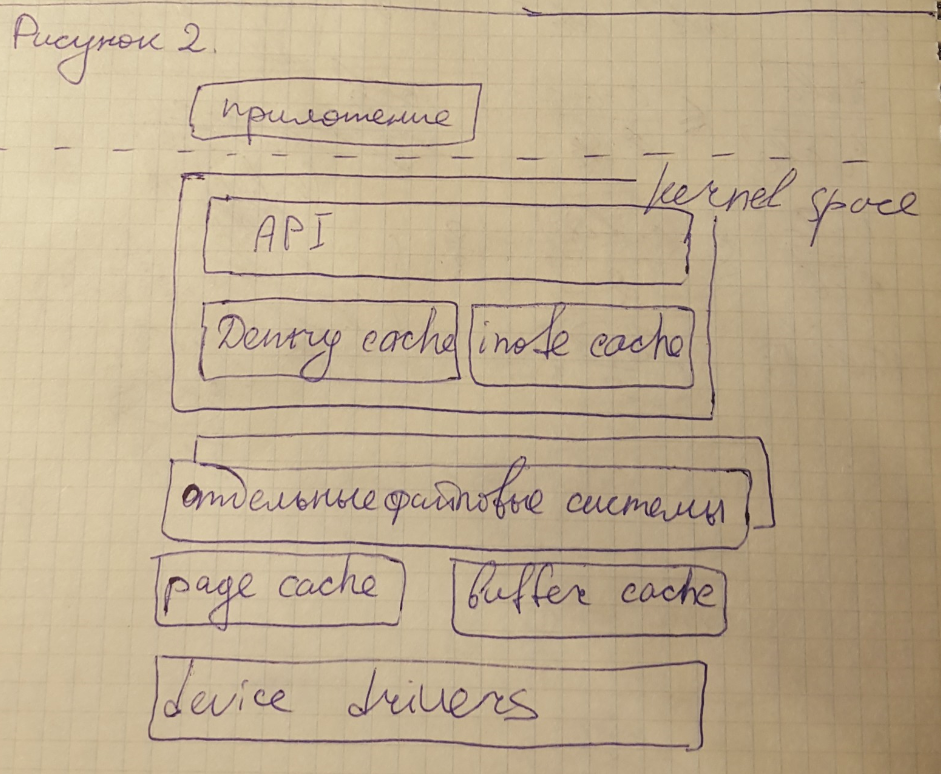
\includegraphics[width=\textwidth]{pic/2.png}
  \caption{Высокоуровневый взгляд на уровни vfs.}
\end{figure}

\section{Файловая система proc}

Unix поддерживает виртуальную файловую систему proc. В зависимости от версии ядра, м.б. procfs. Не является монтируемой ФС. Это пример виртуально ФС. Это интерфейс ядра, позволяющий приложениям читать и изменять данные в адресном пространстве других процессов, управлять прцоессами, получать информацию о процессах и ресурсах используемых процессами путем использования стандартного интерфейса ФС и системных вызовов. Следует, что управление доступом к адресному пространству осуществляется с помощью обычных прав доступа, а именно чтение/запись/выполнение. По умолчанию запись/чтение файлов proc разрешены только для владельцев. В  ФС proc данные о каждом процессе хранятся в поддиректории $/proc/<PID>$
В поддиректории процесса находятся файлы и поддиректория, содержащие данные о процессе. 

\begin{table}[H]
\begin{tabular}{|l|l|l|}
\hline
элемент & тип & содержание \\
\hline
cmdline & файл & указатель на dir процесса \\
cwd & символ ссылка & указатель на dir процесса\\
environ & файл & список окружения процесса\\
exe & символ ссылка & указывает на образ процесса (на файл)\\
fd & директория & ссылки на файлы, открытые процессом\\
root & символ. ссылка & на корень ф.сист. процесса\\
stat & файл & информация о прцоессе.\\
\hline
\end{tabular}
\end{table}

Нужная информация генерируется динамически, когда соответствующий файл читается. 

Есть другой способ получения инфомации о процессе, это использование ссылки self. Если набрать $/proc/self$  то в этой поддиректории будет обнаружен каталог с данными.

\lstinputlisting[language=c, caption=Пример печатающий информацию об окружении]{listing/4.c} 
